\documentclass[12pt]{beamer}
\usetheme{Boadilla}
\usepackage{booktabs}
\usepackage{enumitem}
\usepackage{tikz}

\newcommand{\E}{\mathbb{E}}
\usefonttheme{professionalfonts}
\usepackage{pgfplots}
\renewcommand{\arraystretch}{1.25}
\usetikzlibrary{trees}
\title[ECON2843]{Lecture 13}
\subtitle{Part 3 Estimation and Hypothesis Test}
\date{}
\usepackage{amsmath,amssymb,mathtools,wasysym}
\begin{document}
	\begin{frame}
		\titlepage
	\end{frame}
	\begin{frame}
		\vspace{1cm}
		\centering
		{\color{blue}\large Continue our talk about interval estimation...}
	\end{frame}
\begin{frame}
	\frametitle{90\% Confidence Interval for $\mu$}
	
	\begin{equation*}
		P\left(\bar{X} - 1.645\frac{\sigma}{\sqrt{n}} < \mu < \bar{X} + 1.645\frac{\sigma}{\sqrt{n}}\right) = 0.90
	\end{equation*}
	

	\begin{itemize}[label={\color{blue}$\blacktriangleright$}]
		\item We get a 90\% confidence interval by using 1.645:
	\end{itemize}
	

	\begin{equation*}
		\bar{X} \pm 1.645\frac{\sigma}{\sqrt{n}} = \left(\bar{X} - 1.645\frac{\sigma}{\sqrt{n}}, \bar{X} + 1.645\frac{\sigma}{\sqrt{n}}\right)
	\end{equation*}
	
\end{frame}
\begin{frame}
	\frametitle{\textcolor{blue}{99\% Confidence Interval for $\mu$}}
	
	\begin{equation*}
		P\left(\bar{X} - 2.575\frac{\sigma}{\sqrt{n}} < \mu < \bar{X} + 2.575\frac{\sigma}{\sqrt{n}}\right) = 0.99
	\end{equation*}
	
	
	\begin{itemize}[label={\color{blue}$\blacktriangleright$}]
		\item We get a 99\% confidence interval by using 2.575:
	\end{itemize}
	
	
	\begin{equation*}
		\bar{X} \pm 2.575\frac{\sigma}{\sqrt{n}} = \left(\bar{X} - 2.575\frac{\sigma}{\sqrt{n}}, \bar{X} + 2.575\frac{\sigma}{\sqrt{n}}\right)
	\end{equation*}
	
\end{frame}

\begin{frame}
	\frametitle{\textcolor{blue}{100(1 - $\alpha$)\% Confidence Interval for $\mu$}}
	
	\begin{equation*}
		P\left(\bar{X} - z_{\frac{\alpha}{2}}\frac{\sigma}{\sqrt{n}} < \mu < \bar{X} + z_{\frac{\alpha}{2}}\frac{\sigma}{\sqrt{n}}\right) = 1 - \alpha
	\end{equation*}
	
	\begin{itemize}[label={\color{blue}$\blacktriangleright$}]
		\item A 100(1 - $\alpha$)\% confidence interval for $\mu$ when $\sigma^2$ is known is given by:
	\end{itemize}
	
	\begin{equation*}
		\bar{X} \pm z_{\frac{\alpha}{2}}\frac{\sigma}{\sqrt{n}} = \left(\bar{X} - z_{\frac{\alpha}{2}}\frac{\sigma}{\sqrt{n}}, \bar{X} + z_{\frac{\alpha}{2}}\frac{\sigma}{\sqrt{n}}\right)
	\end{equation*}
	
\end{frame}
\begin{frame}
	\frametitle{\textcolor{blue}{100(1 - $\alpha$)\% Confidence Interval for $\mu$}}
	
	\begin{itemize}[label={\color{blue}$\blacktriangleright$}]
		\item $\bar{X} - z_{\frac{\alpha}{2}}\frac{\sigma}{\sqrt{n}}$ is called the \textbf{lower confidence limit}.
		
		\item $\bar{X} + z_{\frac{\alpha}{2}}\frac{\sigma}{\sqrt{n}}$ is called the \textbf{upper confidence limit}.
		
		\item 1 - $\alpha$ is called the \textbf{confidence level} and is equal to the proportion of intervals under repeated sampling that contain the population mean.
		
		\item $\pm z_{\frac{\alpha}{2}}$ are the points which cut off an area of $\frac{\alpha}{2}$ in the tails of the standard normal PDF and leave an area of 1 - $\alpha$ in the middle.
	\end{itemize}
	
\end{frame}
\begin{frame}
	\frametitle{100(1 - $\alpha$)\% Confidence Interval for $\mu$}
	\centering
	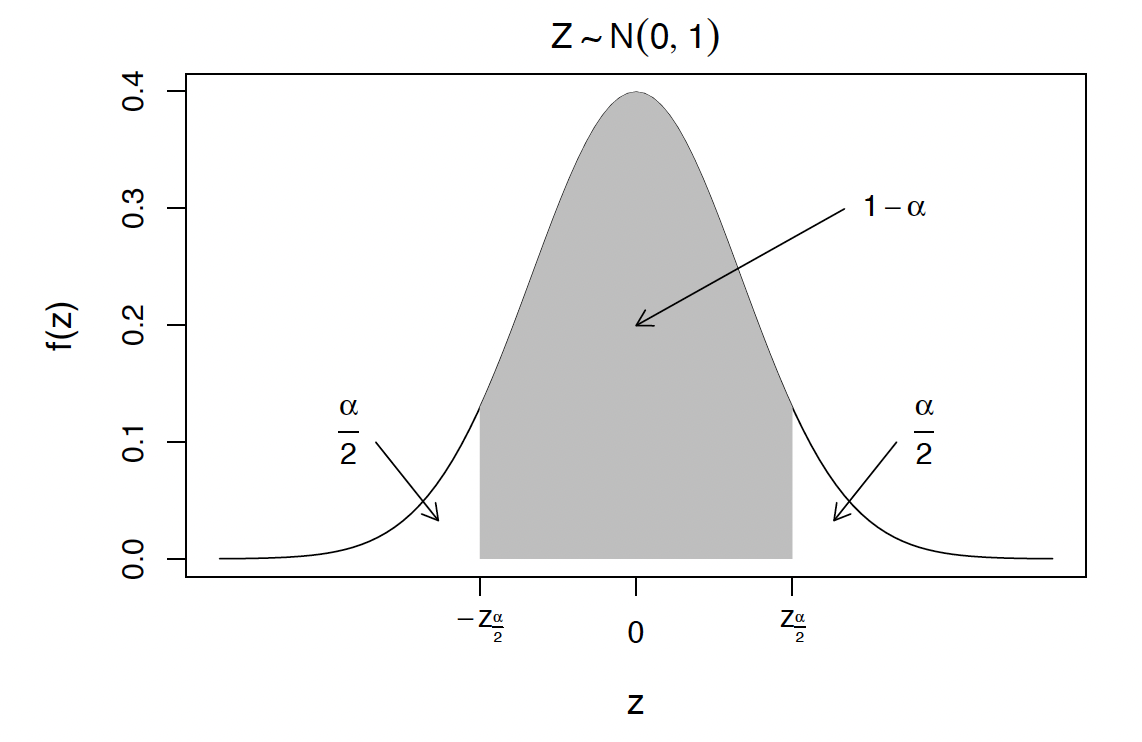
\includegraphics[width=11cm]{table.png}
\end{frame}
\begin{frame}
	\frametitle{\textcolor{blue}{Factors Affecting the Confidence Interval}}
	
	\begin{equation*}
		\left(\bar{X} - z_{\frac{\alpha}{2}}\frac{\sigma}{\sqrt{n}}, \bar{X} + z_{\frac{\alpha}{2}}\frac{\sigma}{\sqrt{n}}\right)
	\end{equation*}
	
	\begin{itemize}[label={\color{blue}$\blacktriangleright$}]
		\item Population variance: Larger variation in the random variable widens the interval.
		
		\item Sample size: As $n$ gets bigger, the interval gets narrower.
		
		\item Confidence level: Increasing confidence level will make the interval wider. For example, to go from 95\% to 99\%, we change 1.96 to 2.575, which widens the interval.
	\end{itemize}
	
\end{frame}
\begin{frame}
	\frametitle{\textcolor{blue}{Interpreting a Confidence Interval}}
	
	\begin{itemize}[label={\color{blue}$\blacktriangleright$}]
		\item Remember that it is the \textit{interval} that is random and therefore changes from sample to sample.
		
		\item The population mean $\mu$ is a fixed and constant value - it is either within the interval or not.
		
		\item You should interpret a 100(1 - $\alpha$)\% confidence interval as saying ``in repeated sampling, 100(1 - $\alpha$)\% of such intervals created would contain the true population mean''.
	\end{itemize}
	
\end{frame}
\begin{frame}
	\frametitle{\textcolor{blue}{Interpreting a Confidence Interval}}
	\centering
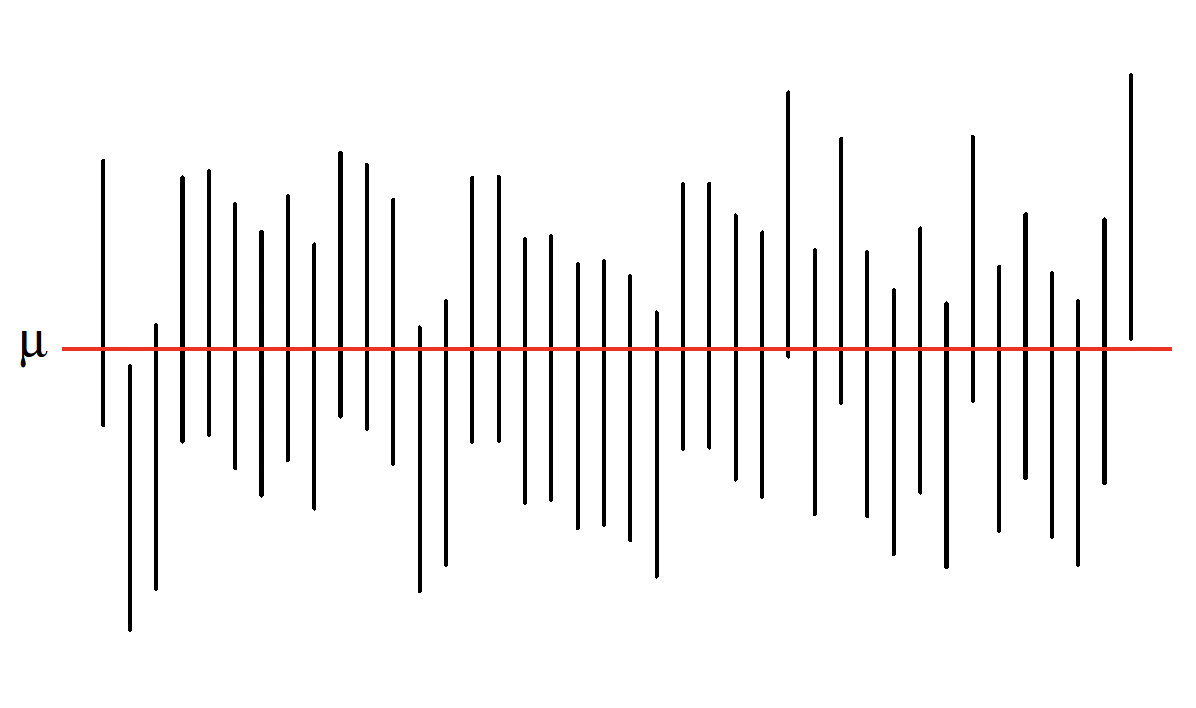
\includegraphics[width=11cm]{interval.png}

	
\end{frame}
\begin{frame}
	\frametitle{Example 1}
	\begin{itemize}[label={\color{blue}$\blacktriangleright$}]
	\item The average height of a sample of 25 men is found to be 178cm. Assume that the standard deviation of male heights is known to be 10cm, and that heights follow a normal distribution.
	
		\begin{enumerate}[label=\textcolor{blue}{(\alph*)}]
		\item Find a 95\% confidence interval for the population mean height.
		\item To what confidence level does an interval of $(174.71, 181.29)$ correspond?
	\end{enumerate}
\end{itemize}
	
\end{frame}

\begin{frame}
	\frametitle{\textcolor{blue}{Solution - Part (a)}}
	
	\begin{itemize}[label={\color{blue}$\blacktriangleright$}]
		\item For a 95\% confidence interval, we know that 
		$z_{\frac{\alpha}{2}} = z_{0.025} = 1.96$. Therefore:
		
		
		\begin{align*}
			\bar{X} \pm z_{\frac{\alpha}{2}}\frac{\sigma}{\sqrt{n}} &= 178 \pm 1.96 \times \frac{10}{\sqrt{25}} \\
			&= (174.08, 181.92)
		\end{align*}
		
		
		\item So, in repeated sampling, we would expect 95\% of the intervals created this way to contain $\mu$.
	\end{itemize}
	
\end{frame}

\begin{frame}
	\frametitle{\textcolor{blue}{Solution - Part (b)}}
	
	\begin{itemize}[label={\color{blue}$\blacktriangleright$}]
		\item From the lower confidence limit, we get:
		
		
		\begin{align*}
			\bar{X} - z_{\frac{\alpha}{2}}\frac{\sigma}{\sqrt{n}} &= 174.71 \\
			178 - z_{\frac{\alpha}{2}}\frac{10}{\sqrt{25}} &= 174.71 \\
			z_{\frac{\alpha}{2}} &= \frac{\sqrt{25}}{10} \times (178 - 174.71) \\
			z_{\frac{\alpha}{2}} &= 1.645
		\end{align*}
		
		
		\item From the $z$-tables, we know that $\frac{\alpha}{2} = 0.05$ so this corresponds to a $100(1 - \alpha) = 90\%$ confidence interval.
	\end{itemize}
	
\end{frame}
\begin{frame}
	\frametitle{Backward - How large should sample size be?}
	\begin{itemize}[label={\color{blue}$\blacktriangleright$}]
		\item Suppose that before we gather data, we know that we want to get an estimate within a certain distance of the true population value.
		\item We can use the CLT to find the minimum sample size required to meet this condition, if the population standard deviation is known.
		
	\end{itemize}
	
\end{frame}
\begin{frame}
	\frametitle{Example 2}
	\begin{itemize}[label={\color{blue}$\blacktriangleright$}]
		\item I time my morning bus trips to work, and get an average of 35 minutes. Assuming that the standard deviation of times is known to be 5 minutes, I want to estimate the true population mean length to within 3 minutes, with {\bf 99\% certainty}. How many bus trips should I time for calculating my average?
		
	\end{itemize}
	
\end{frame}
\begin{frame}
	\frametitle{\textcolor{blue}{Solution}}
	
	\begin{itemize}[label={\color{blue}$\blacktriangleright$}]
		\item Step 1: Set up the required equation, then standardize:
		
		
		\begin{align*}
			P(|\bar{X} - \mu| < 3) &= 0.99 \\
			P(-3 < \bar{X} - \mu < 3) &= 0.99 \\
			P\left(-\frac{3}{\frac{\sigma}{\sqrt{n}}} < \frac{\bar{X} - \mu}{\frac{\sigma}{\sqrt{n}}} < \frac{3}{\frac{\sigma}{\sqrt{n}}}\right) &= 0.99 \\
			P\left(-\frac{3}{\frac{5}{\sqrt{n}}} < Z < \frac{3}{\frac{5}{\sqrt{n}}}\right) &= 0.99
		\end{align*}
	\end{itemize}
	
\end{frame}

\begin{frame}
	\frametitle{\textcolor{blue}{Solution}}
	
	\begin{itemize}[label={\color{blue}$\blacktriangleright$}]
		\item Step 2: We know $P(-2.575 < Z < 2.575) = 0.99$. Therefore solve for $n$:
		
		\begin{align*}
			\frac{3}{\frac{5}{\sqrt{n}}} &= 2.575 \\[10pt]
			\sqrt{n} &= 2.575 \times \frac{5}{3} \\[10pt]
			n &= 18.42 \approx 19
		\end{align*}
		
		
		\item I need to time at least 19 (round up!) bus trips in order to derive a 99\% CI that estimates $\mu$ to within 3 minutes.
	\end{itemize}
	
\end{frame}
\begin{frame}
	\vspace{1cm}
	\centering
	{\color{blue}\large Hypothesis Test}
\end{frame}
\begin{frame}
	\frametitle{Statistical Inference}
	
	\begin{itemize}[label={\color{blue}$\blacktriangleright$}]
		\item Estimation (last time):
		\begin{itemize}[label={\color{blue}$\blacktriangleright$}]
			\item Draw inferences about a population by selecting a sample and \emph{estimating} population parameters (point and interval estimators).
		\end{itemize}
		
		\item Hypothesis testing (this time):
		\begin{itemize}[label={\color{blue}$\blacktriangleright$}]
			\item Draw inferences about a population by making a \emph{claim} or \emph{hypothesis} about a population parameter and testing whether the hypothesis is supported by the sample.
		\end{itemize}
		\item They are different!
	\end{itemize}
	
\end{frame}
\begin{frame}
	\frametitle{\color{blue}Let's Go Bowling!}
	
	\begin{itemize}[label={\color{blue}$\blacktriangleright$}]
		\item Suppose we all go bowling.
		\item Before the game, I claim that my average bowling score is 150 (but you think it's lower).
		\item Over 10 games, my average score turns out to be 80.
		\item Do you believe my claim?
	\end{itemize}
	
\end{frame}
\begin{frame}
	\frametitle{\color{blue}Let's Go Bowling!}
	
	\begin{itemize}[label={\color{blue}$\blacktriangleright$}]
		\item Assume bowling scores are normally distributed.
		\item The population:
		\begin{itemize}
			\item An infinite number of my bowling scores.
		\end{itemize}
		\item The claim/hypothesis:
		\begin{itemize}
			\item That the population mean is 150 ($\mu = 150$).
		\end{itemize}
		\item The sample and sample statistic:
		\begin{itemize}
			\item Bowling scores from 10 games and $\bar{X} = 80$.
		\end{itemize}
		\item Does the sample and sample statistic support my hypothesis?
		\item How can we decide?
	\end{itemize}
	
\end{frame}

	
	\begin{frame}
		\frametitle{\color{blue}One Possible Approach}
		
		\begin{itemize}[label={\color{blue}$\blacktriangleright$}]
			\item Assume that the hypothesis is true (i.e, my true bowling average is 150).
			\item Choose some (lower) cut-off score. (Chosen by person)
			\item Compare my sample mean bowling score from 10 games to this cut-off.
			\item If my sample mean is below the cut-off, reject the hypothesis.
		\end{itemize}
		
	\end{frame}
	
	\begin{frame}
	\frametitle{\color{blue}One Possible Approach}
	
	\begin{itemize}[label={\color{blue}$\blacktriangleright$}]
		\item For example, we might choose a cut-off value of $c = 120$:
	\end{itemize}
	\centering
	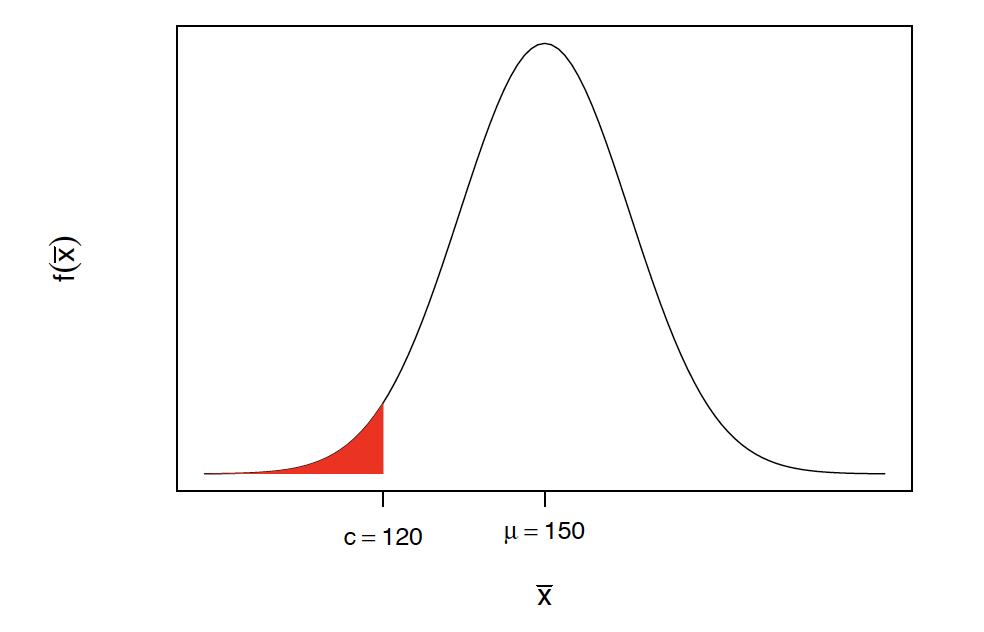
\includegraphics[width=11cm]{bowling1.png}
\end{frame}
	\begin{frame}
	\frametitle{\color{blue}One Possible Approach}
	
	\begin{itemize}[label={\color{blue}$\blacktriangleright$}]
		\item To be even more confident in our decision to reject the hypothesis, we could lower our cut-off:
	\end{itemize}
	\centering
	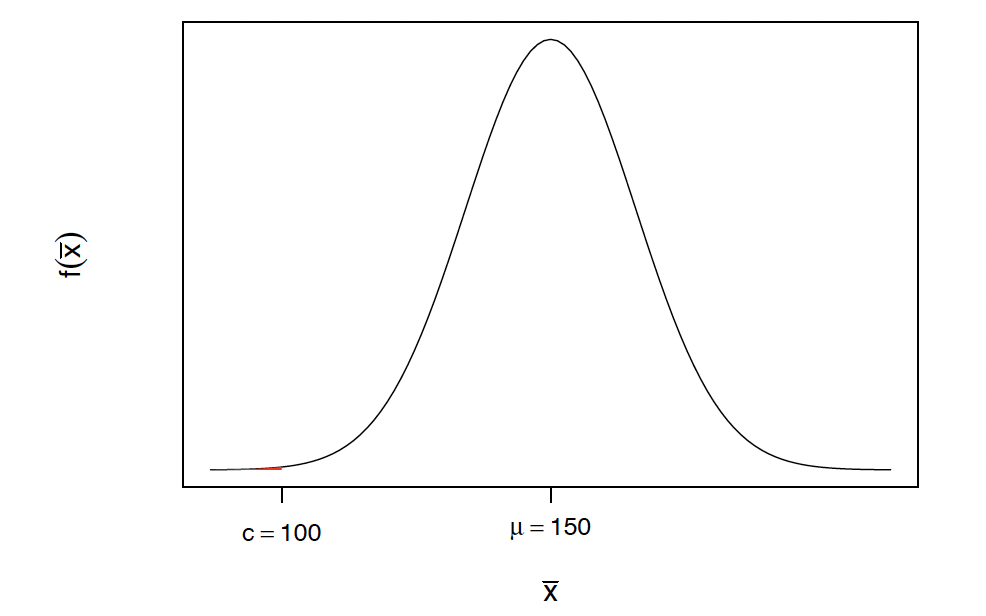
\includegraphics[width=11cm]{bowling2.png}
\end{frame}

\begin{frame}
	\frametitle{\color{blue}1. Hypotheses}
	
	\begin{itemize}[label={\color{blue}$\blacktriangleright$}]
		\item We always test between two hypotheses, the \emph{null hypothesis} and the \emph{alternative hypothesis}.
		\item We start by assuming the null hypothesis is true.
		\item Goal is to determine if there is enough evidence to conclude that the alternative hypothesis is true.
		\item So, based on our sample data, we make one of two decisions:
		\begin{enumerate}[label=\textcolor{blue}{(\alph*)}]
			\item \emph{Reject} the null hypothesis (enough evidence in favour of the alternative hypothesis). Or,
			\item \emph{Fail to reject} the null hypothesis (not enough evidence in favour of the alternative hypothesis).
		\end{enumerate}
	\end{itemize}
	
\end{frame}
\begin{frame}
	\frametitle{\color{blue}Null Hypothesis}
	
	\begin{itemize}[label={\color{blue}$\blacktriangleright$}]
		\item The \textbf{null hypothesis} ($H_0$) usually corresponds to a default claim about a population parameter.
		\item For hypothesis tests concerning a \emph{single} population parameter, almost always involves an ``$=$'' sign.
		\item Bowling example:
		\begin{itemize}[label={\color{blue}$\blacktriangleright$}]
			\item $H_0 : \mu = 150$, i.e., mean bowling score is 150.
		\end{itemize}
	\end{itemize}
	
\end{frame}

\begin{frame}
	\frametitle{\color{blue}Alternative Hypothesis}
	
	\begin{itemize}[label={\color{blue}$\blacktriangleright$}]
		\item The \textbf{alternative hypothesis} ($H_1$) usually represents a claim about the population parameter that we are trying to prove.
		\item Generally involves a ``$<$'', ``$>$'' or ``$\neq$'' sign.
		\item Bowling example:
		\begin{itemize}
			\item $H_1 : \mu < 150$, i.e., mean bowling score is less than 150.
		\end{itemize}
	\end{itemize}
	
\end{frame}

\end{document}